\documentclass[10pt]{beamer}
\usepackage{mathtools}
\usetheme[
%%% option passed to the outer theme
%    progressstyle=fixedCircCnt,   % fixedCircCnt, movingCircCnt (moving is deault)
progressstyle=fixedCircCnt
  ]{Feather}
\usepackage[utf8]{inputenc}
\usepackage[english]{babel}
\usepackage[T1]{fontenc}
\usepackage{helvet}
\usepackage{color}
\usepackage[
	backend=biber,
	style=numeric,
	citestyle=authoryear,
	maxnames=10,
]{biblatex}
\usepackage{booktabs}

\addbibresource{mybib.bib}
\renewbibmacro{in:}{}

\definecolor{blue}{HTML}{1f77b4}
\definecolor{orange}{HTML}{ff7f0e}
\definecolor{green}{HTML}{2ca02c}
\definecolor{red}{HTML}{d62728}
\definecolor{purple}{HTML}{9467bd}
\definecolor{brown}{HTML}{8c564b}

\newcommand{\R}{\mathbb{R}}
\newcommand{\dd}{{\rm d}}

\title[%
	MSIAM M2 Thesis: Extreme quantile Bayesian estimators]
{%
	\textbf{MSIAM M2 Thesis: Extreme quantile Bayesian inference}}

\subtitle[]{}

\author[Tony Zheng]{Tony Zheng}

%Supervisors: \\
%Anne Dutfoy (EDF R\&D) \\
%Stephane Girard (Inria Grenoble Rhone-Alpes) \\
%Julyan Arbel (Inria Grenoble Rhone-Alpes)

\institute[]{}

\date{\today}

\begin{document}
%
{\1\begin{frame}[plain,noframenumbering]\titlepage\end{frame}}
%
%-------------------------------------------------------
%
\begin{frame}{Problem}{}
%
\begin{itemize}
	\item[] \textbf{Given:}
		\begin{itemize}
			\item Observations of some variable.
			\item Expert who has knowledge about this process.
		\end{itemize}
	\item[] \textbf{Goal:} How can we incorporate expert opinion
		to model quantiles of maxima?
	\item[] \textbf{Applications:} Environmental variables such as
	rainfall, wind speed, river discharge etc.
\end{itemize}
%
\end{frame}
%
%-------------------------------------------------------
%
\begin{frame}{Extreme value modelling 1}{}
%
\begin{itemize}
	\item Maxima are often modelled with the
		generalised extreme value (GEV)
		distribution with parameters $\mu, \sigma > 0, \xi \neq 0$.
	\item Its CDF is
		\begin{align*}
			F(x) =
				\exp\left(-\left\{1 + \xi
				\left(\frac{x - \mu}{\sigma}\right)\right\}_+
				^ {-\frac{1}{\xi}}\right) \,,
		\end{align*}
		where $\{x\}_+ = \max(x, 0)$.
\end{itemize}
%
\end{frame}
%
%-------------------------------------------------------
%
\begin{frame}{Extreme value modelling 2}{}
%
\begin{itemize}
	\item The GEV model can be generalised to a
		non-homogeneous Poisson point process
		with the same parameters.
	\item This model considers exceedances of a certain threshold as events
		occurring with intensity function
		\begin{align*}
			\lambda(x) =
			\frac{1}{\sigma}
				\left\{1 + \xi \left(\frac{x - \mu}{\sigma}\right)\right\}_+
				^ {-\frac{\xi + 1}{\xi}} \,.
		\end{align*}
	\item Advantage: uses all observations above some threshold,
		not just block maxima.
\end{itemize}
%
\end{frame}
%
%-------------------------------------------------------
%
\begin{frame}{Data}{}
%
\begin{figure}
	\centering
	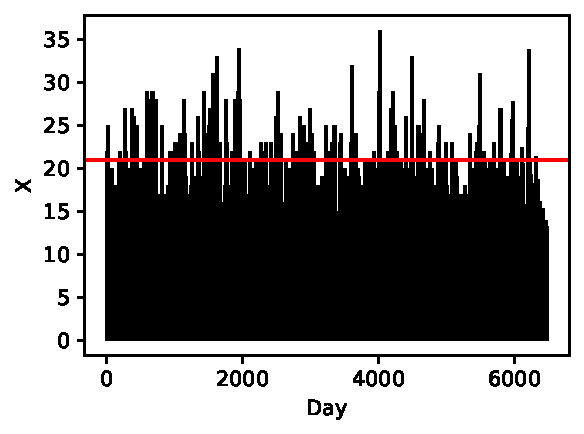
\includegraphics[width=0.5\linewidth]{plots/data.pdf}
\end{figure}
%
\begin{itemize}
	\item Daily observations of average wind speed
		at Tours, France from 1981 to 2011.
	\item Chosen threshold in red.
	\item Goal: estimate quantiles (return levels) of the annual maxima.
\end{itemize}
%
\end{frame}
%
%-------------------------------------------------------
%
\begin{frame}{Bayesian inference}{}
%
\begin{itemize}
	\item Bayes' theorem:
		\begin{align*}
			\pi(\mu, \sigma, \xi \mid \mathbf{x}) \propto {\cal L}(\theta \mid \mathbf{x}) \pi(\mu, \sigma, \xi) \,,
		\end{align*}
		where ${\cal L}$ is the likelihood of the Poisson point process model
		and $\pi$ is a prior on the parameters.
	\item Prior elicitation:
		\begin{align*}
			\text{Expert opinion} \longrightarrow \pi(\mu, \sigma, \xi) \,.
		\end{align*}
	\item Maximum entropy principle: given some constraints,
		choose a distribution with PDF $f$ which maximises the Shannon entropy
		%
		\begin{align*}
			{\cal E}(f) \coloneqq -\int_0^{+\infty} f(x) \log(f(x)) \, \dd x \,.
		\end{align*}
\end{itemize}
%
\end{frame}
%
%-------------------------------------------------------
%
\begin{frame}{Reparametrisation}{}
%
\begin{itemize}
	\item Let $q_1, q_2, q_3$ be the quantiles of annual maxima
		with probabilities $p_1 < p_2 < p_3$ respectively.
	\item There is an invertible transformation
		$(q_1, q_2, q_3) \to (\mu, \sigma, \xi)$.
	\item It is much easier for an expert to specify information about
	the quantiles than $\mu, \sigma, \xi$.
	\item The problem becomes:
		\begin{align*}
			\text{Expert opinion} \longrightarrow \pi(q_1, q_2, q_3) \,.
		\end{align*}
\end{itemize}
%
\end{frame}
%
%-------------------------------------------------------
%
\begin{frame}{Order constraint on quantiles}{}
%
\begin{itemize}
	\item The quantiles must satisfy the order constraint
		$q_1 < q_2 < q_3$.
	\item Solution 1: Positive priors on each quantile difference
		\begin{align*}
			\tilde{q}_1 &\coloneqq q_1 \,,\\
			\tilde{q}_2 &\coloneqq q_2 - q_1 \,,\\
			\tilde{q}_3 &\coloneqq q_3 - q_2 \,,
		\end{align*}
		with independent copula (\cite{coles1996}).
	\item Solution 2: Positive priors on each quantile, with some copula
		which satisfies order constraint.
		We choose the copula with maximum entropy,
		which has been derived in \cite{butucea2018}.
\end{itemize}
%
\end{frame}
%
%-------------------------------------------------------
%
\begin{frame}{Expert specification}{}
%

%
\begin{itemize}
	\item In both solutions, we need to construct three positive distributions
		from the expert's opinion.
	\item We consider the case where the expert specifies
		the mean and variance of each distribution.
	\item In this case, the maximum entropy distribution
		is a truncated normal distribution.
\end{itemize}

%
%
\end{frame}
%
%-------------------------------------------------------
%
\begin{frame}{Incomplete information}{}
%
\begin{itemize}
	\item So far, the expert has given information on $k = 3$
		quantiles/quantile differences. 
	\item We will also consider case $k = 2$, for which the expert
		specifies information on $2$ quantiles/quantile differences.
	\item We use a reparametrisation
		$(q_1, q_2, \sigma) \to (\mu, \sigma, \xi)$,
		and place a uniform prior on $\log \sigma$.
\end{itemize}
%
\end{frame}
%
%-------------------------------------------------------
%
\begin{frame}{Results}{}
%
\begin{figure}
	\centering
	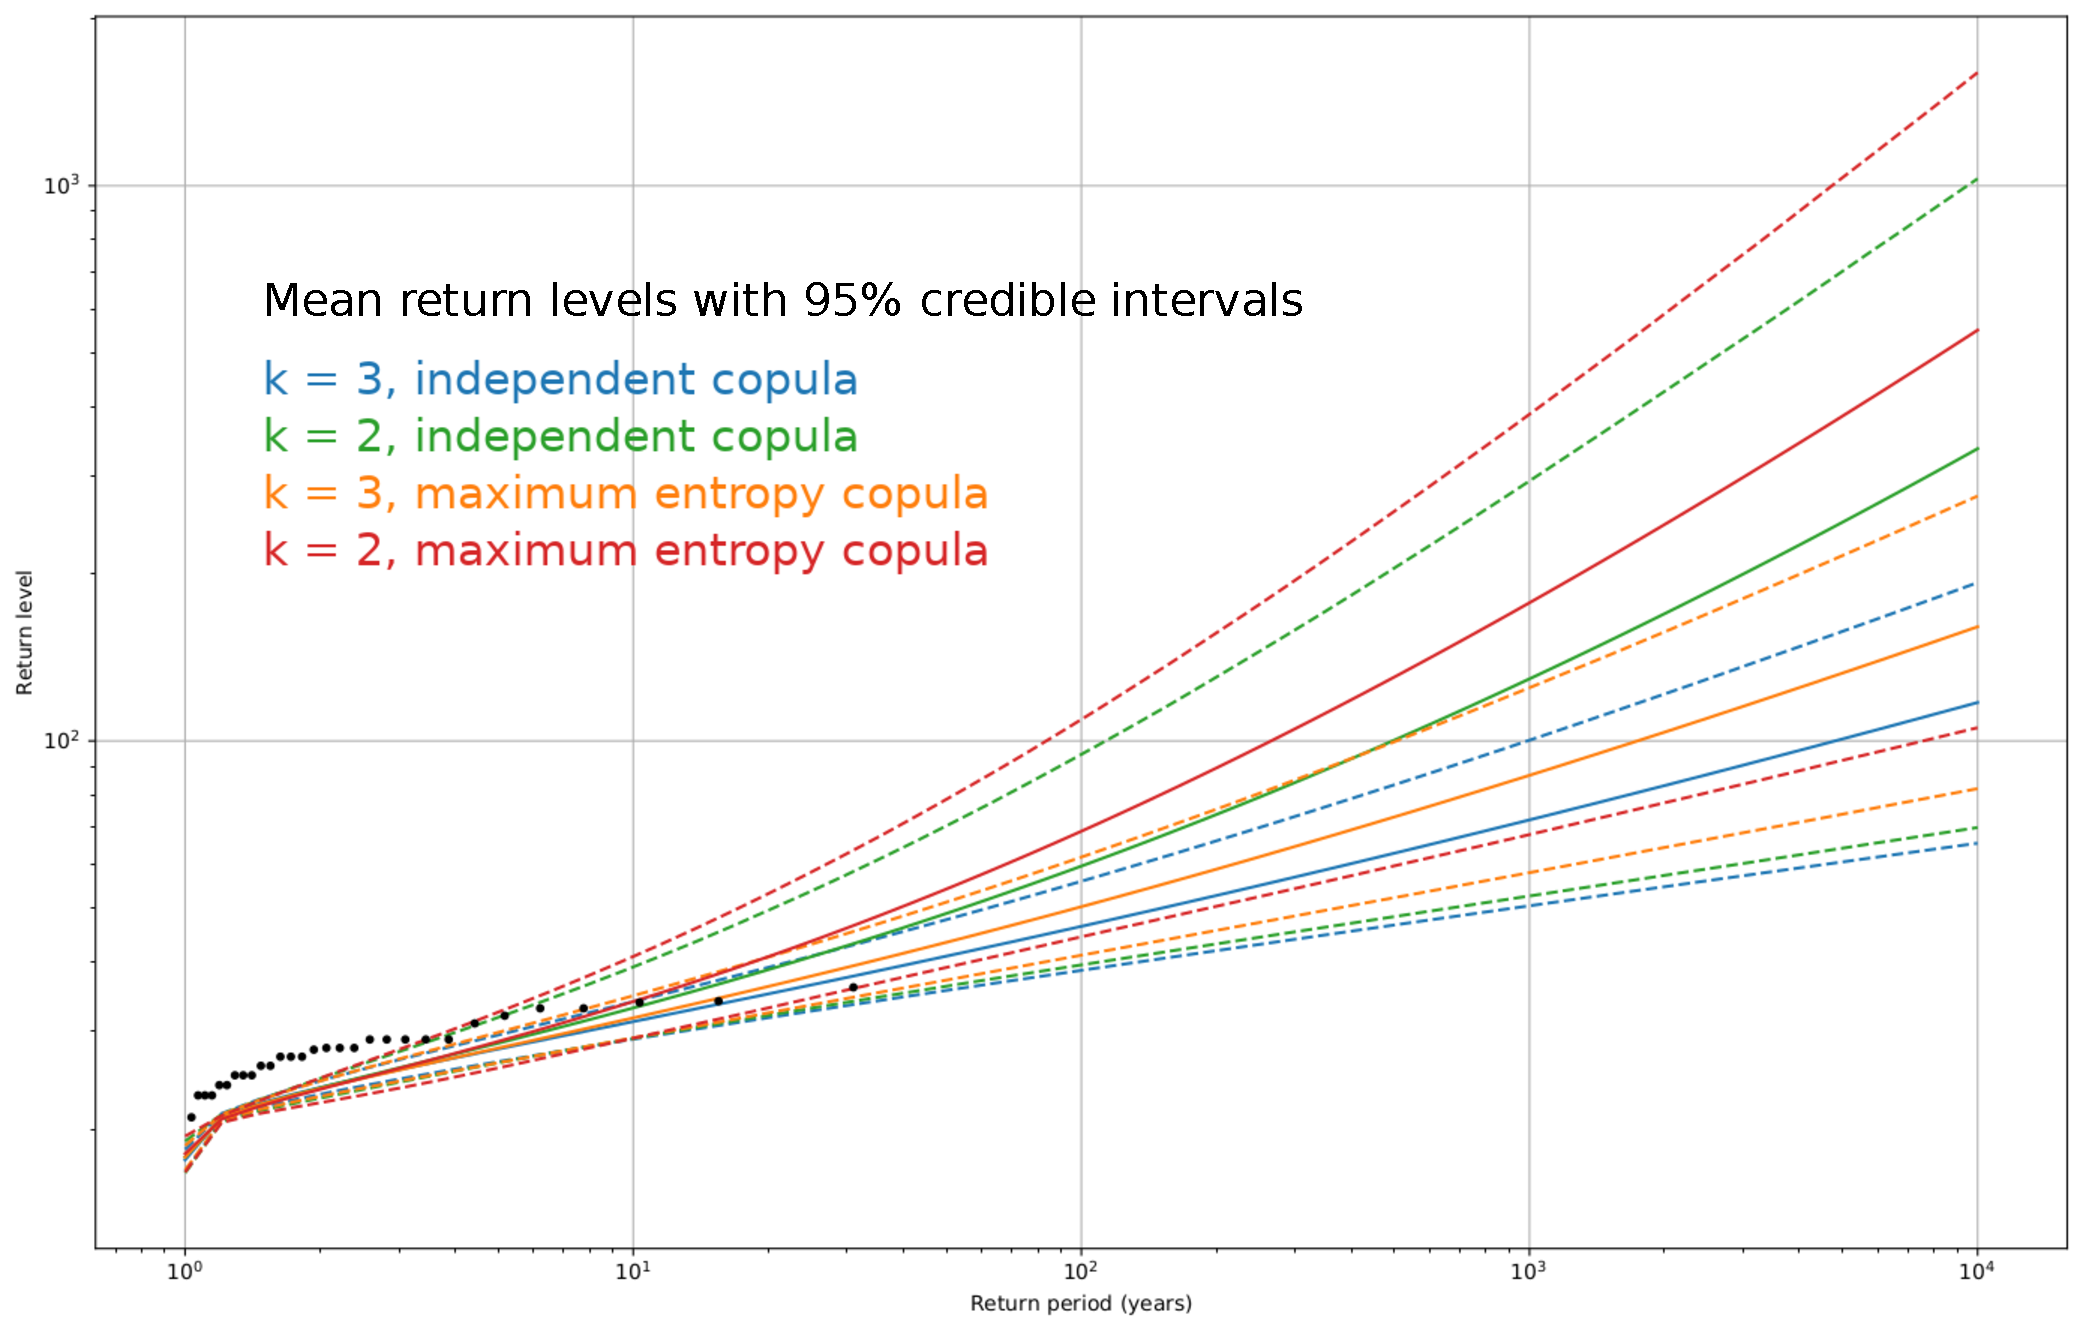
\includegraphics[width=\linewidth]{plots/rl_text.pdf}
\end{figure}
%
\end{frame}
%
%-------------------------------------------------------
%
\begin{frame}{Bibliography}{}
%
\printbibliography
\end{frame}
%
%-------------------------------------------------------
%
\end{document}